% The beamer class automatically loads some other LATEX packages, including
% xcolor, amsmath, amsthm, calc, geometry, hyperref, extsizes.
% color predefined:red, blue, green, cyan, magenta, yellow, black, darkgray, gray,
% lightgray, orange, violet, purple, brown
% \documentclass[11pt]{beamer}
\documentclass[pdf]{beamer}
% aspectratio=1610
% default font size 11pt;8pt, 9pt, 10pt, 11pt, 12pt, 14pt, 17pt, 20pt
% used to print as article
% \documentclass[]{article}
% \usepackage{beamerarticle}

% Antibes, Bergen, Berkeley, Berlin, Boadilla, Copenhagen, Darmstadt, Dresden,
% Frankfurt, Goettingen, Hannover, Ilmenau, Juanlespins, Madrid, Malmoe,
% Marburg, Montpellier, Paloalto, Pittsburgh, Rochester, Singapore, Warsaw
% \usetheme[compress]{Singapore} %title at the top-middle
% \usecolortheme{freewilly}
\usetheme{Boadilla}
% \beamertemplatetransparentcoveredhigh
% \beamertemplatetransparentcovereddynamicmedium

\usepackage[T1]{fontenc}
% \mode<article> % 仅应用于article版本
% {
% \usepackage{beamerbasearticle}
% \usepackage{fullpage}
% \usepackage{hyperref}
% }

%   font theme
%   \usefonttheme[onlymath]{serif}
%   \usefonttheme{structureitalicserif}
%   \usefonttheme{structurebold}
%   \usefonttheme{structuresmallcapsserif}
%   \usepackage{lucidaso} % Lucida Bright (SO Version)
\usefonttheme[onlymath]{serif}
% \usepackage[small]{eulervm} % Euler VM for math font
% \usepackage{helvet}


% color themes:albatross crane beetle dove fly seagull wolverine beaver
% \usecolortheme{fly}
% Outer color themes:whale, seahorse, dolphin
\usecolortheme{whale}
% Inner color themes: lily, orchid,rose
\usecolortheme{orchid}

% rectangles circles inmargin rounded
\useinnertheme{rectangles}
% \useinnertheme[shadow]{rounded}
% infolines miniframes shadow sidebar c smoothtree split tree progressbar
\useoutertheme{progressbar}

% define colors
% \setbeamercolor{uppercol}{fg=white,bg=blue}%
\setbeamercolor{lowercol}{fg=black,bg=gray}%
\xdefinecolor{lavendar}{rgb}{0.8,0.6,1}
\xdefinecolor{olive}{cmyk}{0.64,0,0.95,0.4}
\colorlet{structure}{green!60!black}
% redefine structure color
% \usecolortheme[named=yellow]{structure}
% redefine alert color
% \setbeamercolor{alerted text}{fg=cyan}

\setbeamertemplate{headline}[default]

% \beamertemplateshadingbackground{blue!5}{yellow!10}
% \setbeamertemplate{background canvas}[vertical
% shading][top=blue!30,bottom=white,middle=blue!20,midpoint=.4]
% \setbeamertemplate{sidebar canvas
% left}[horizontal shading][left=white!40!black,right=black]
% \setbeamertemplate{navigation symbols}{}
\mode<beamer>{\setbeamertemplate{blocks}[rounded][shadow=true]}
% transparent,highly dynamic,dynamic,
\setbeamercovered{invisible}
\setbeamercolor{body}{fg=blue!80, bg=black!20}
\setbeamercolor{head}{fg=blue,bg=blue!30}

\setbeamerfont{title}{shape=\slshape,family=\ttfamily,series=\bfseries}

\beamertemplateballitem

\usepackage{wasysym}
\usepackage{pifont}
% \usepackage{textcomp}

% \usepackage{pgf,pgfarrows,pgfnodes,pgfautomata,pgfheaps}


\usepackage{graphicx}

% shadowbox,fbox,Ovalbox,ovalbox,doublebox
\usepackage{fancybox}
\usepackage{fancyvrb}

\usepackage{multimedia}
\usepackage{listings}
\usepackage{boxedminipage}
% \usepackage{babel}
% \usepackage{enumitem}
\usepackage{array}

\usepackage{multirow}

\lstset{
  % 行号
  numbers=left,
  % 背景框
  framexleftmargin=10mm,
  frame=none,
  captionpos=b,
  % 背景色
  % backgroundcolor=\color[rgb]{1,1,0.76},
  % backgroundcolor=\color[RGB]{245,245,244},
  % 样式
  keywordstyle=\bf\color{blue},
  identifierstyle=\bf\color{black!90},
  numberstyle=\color[RGB]{0,192,192}\tiny,
  commentstyle=\it\color[RGB]{0,96,96},
  stringstyle=\rmfamily\slshape\color[RGB]{128,0,0},
  % 显示空格
  showstringspaces=false
}


\title[prune]{Fast Patch Validation via Selective Symbolic Execution}
\author{Cheng Zhang, Hucheng Zhou, Hongxu Chen}
\subject{Test Generation, Regression Testing}
\date[date]{\today}

% \AtBeginSection[]{
%   \frame<handout:0>{
%     \frametitle{Outline}
%     \tableofcontents[current,currentsubsection,shaded]
%   }
%   \addtocounter{framenumber}{-1}%
% }

\hypersetup{pdfpagemode={FullScreen}}
% \hypersetup{pdfstartview={FitH}}

\makeatletter
\newenvironment{CenteredBox}{%
  \begin{Sbox}}{% Save the content in a box
  \end{Sbox}\centerline{\parbox{\wd\@Sbox}{\TheSbox}}}% And output it centered
\makeatother

\newenvironment<>{varblock}[2][\textwidth]{%
  \setlength{\textwidth}{#1}
  \begin{actionenv}#3%
    \def\insertblocktitle{#2}%
    \par%
    \usebeamertemplate{block begin}}
  {\par%
    \usebeamertemplate{block end}%
  \end{actionenv}}

\begin{document}
\frame{\titlepage}
\frame{\maketitle}

\part{Overview}
\frame{\partpage}

\section{Motivation}

\begin{frame}
\frametitle{Patch Validation}
Patches are not always complete
\begin{itemize}
  \item A patch might
    \begin{enumerate}[a]
      \item fail to fix ALL paths w.r.t the bug site
      \item bring about new bugs
    \end{enumerate}
  \item A study shows that about $14.8\% \sim 25\%$ patches are incorrect
  \item Validating patches by \alert{testing} is tedious and time-consuming
\end{itemize}
\pause
\vspace{1pt}
\begin{center}
  \Ovalbox{\textcolor{blue}{How about validating by \alert{symbolic execution}?}}
\end{center}
\end{frame}

\section{Insight}
\begin{frame}
  \frametitle{\secname}
Symbolic Execution
\begin{itemize}
  \item Executes on symbolic value and lets constraint solver compute the condition
  \item \alert{Automatically} generates tests with \alert{higher} coverage and finds \alert{real} bugs
  \item But non-scalable to larger applications due to path explosion
  \end{itemize}
  \pause
  \vspace{1.5pt}
  But for a patch...
\begin{enumerate}
  \item there is no need to check those bugs that are irrelevant
  \item we can only focus on \textcolor{blue}{assertion} bugs
    \vspace{1.5pt}

\begin{center}
  \doublebox{\tiny{Pruning irrelevant paths $\Rightarrow$ Less unnecessay constraints solving $\Rightarrow$ Faster validation for patches}}
\end{center}
\end{enumerate}
\end{frame}

\part{Implementations}
\frame{\partpage}

\section{Main Idea}

\begin{frame}
  \frametitle{\secname}
  \begin{columns}
    \column{.45\textwidth}
  \frametitle{\secname}
  Combine \textcolor{blue}{static pruning} and \textcolor{blue}{symbolic execution}
  \begin{enumerate}
    \item \footnotesize{Pruning code that cannot \emph{reach} from \textcolor{blue}{patch site} and doesn't have influence on \textcolor{blue}{assert site} for bug/patch versions of programs($\Rightarrow$ \alert{rbscope})}
    \item \footnotesize{Linking 2 versions of program into 1 new program, adding symbolic execution semantics for entry function formal argument and global variables and special functions for validating}
  \end{enumerate}
  \pause
    \column{.45\textwidth}
    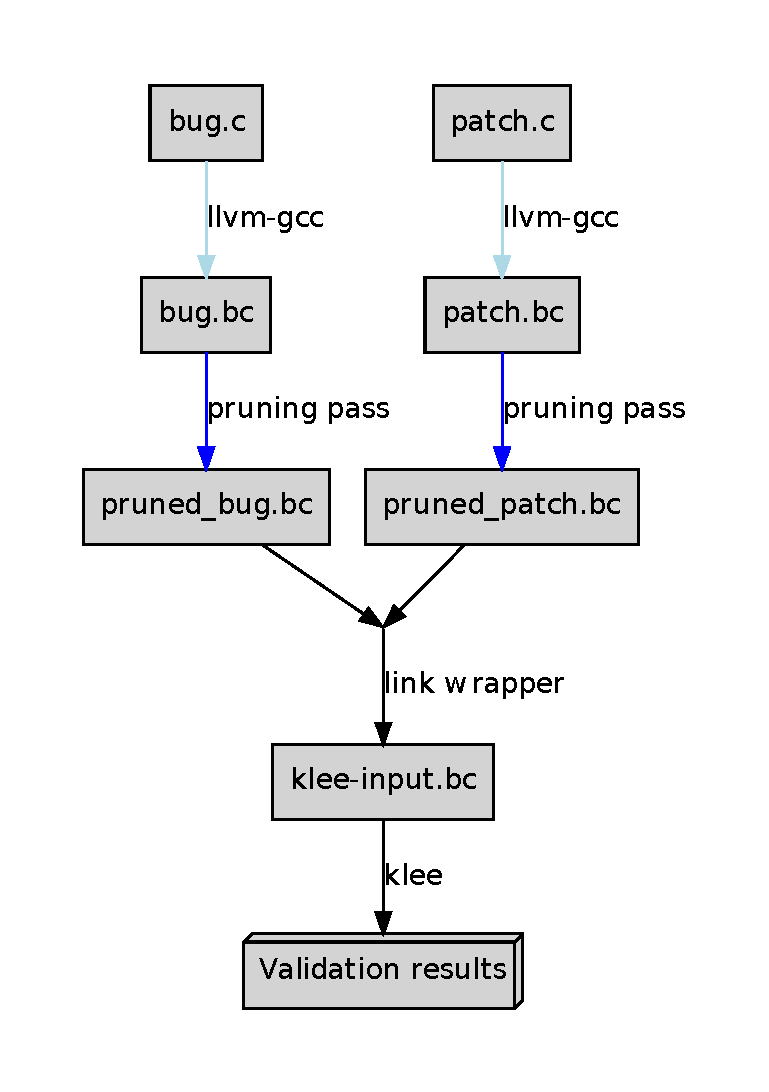
\includegraphics[height=.9\textheight]{fig/whole.pdf}
  \end{columns}
\end{frame}

\section{Pruning}

% \begin{frame}
%   \frametitle{Principles of Pruning}
%   \begin{itemize}
%   \item Pruning should be \alert{conservative} \pause
%   \item Prune as many instructions as possible \pause
%   \item The remaing snippets should be \alert{executable}
%   \end{itemize}
% \end{frame}

\begin{frame}
  \frametitle{Flow Chart for Pruning}
  \begin{center}
    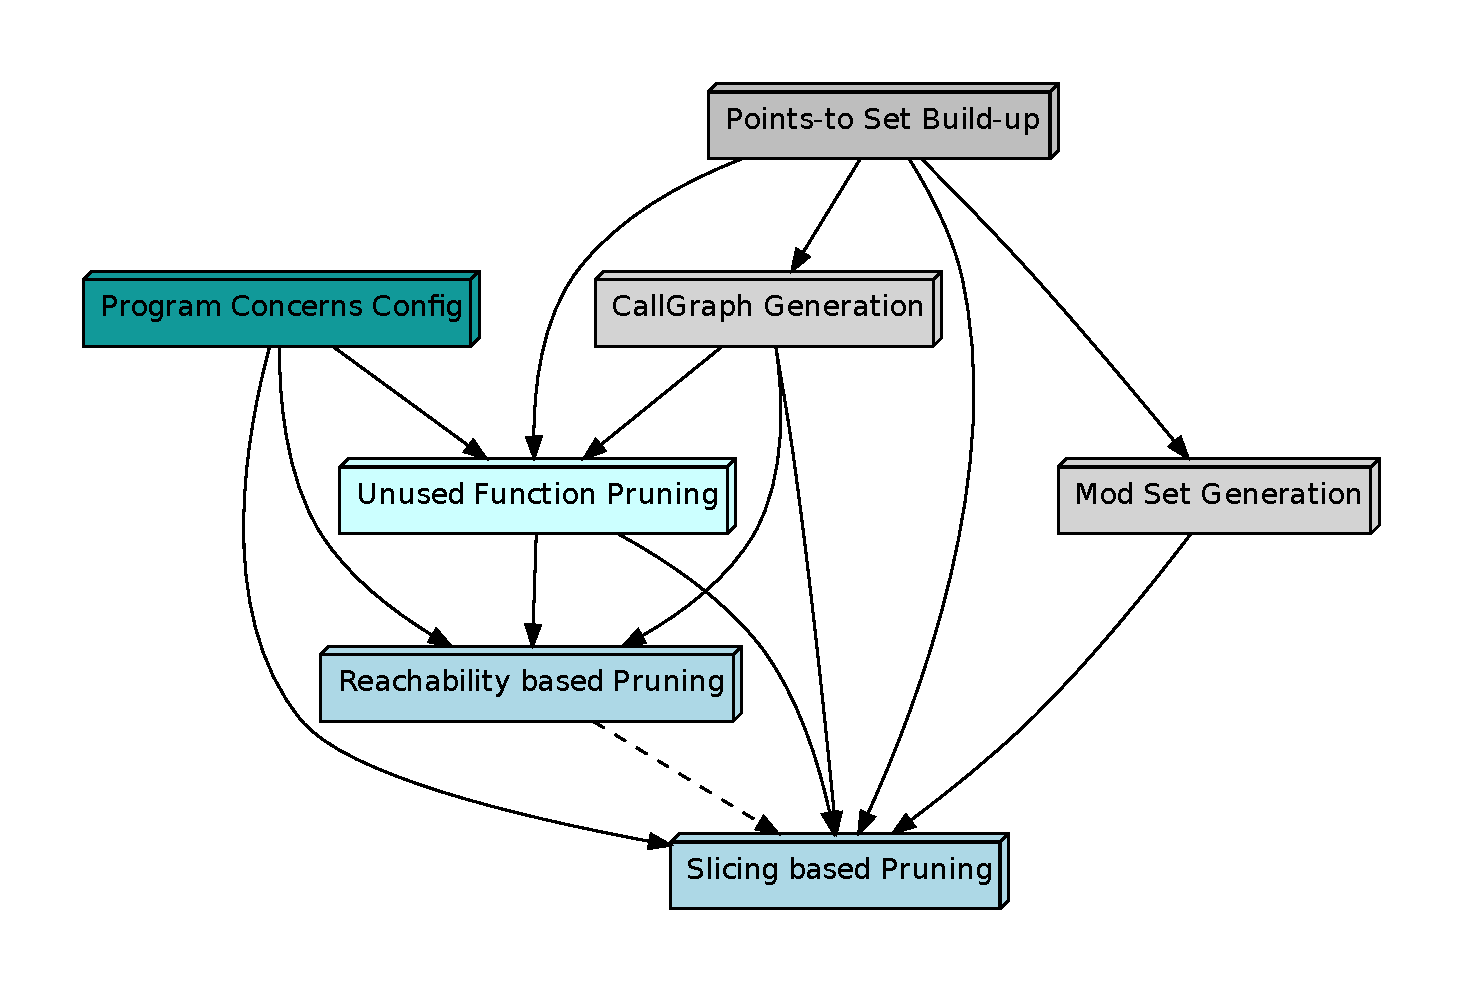
\includegraphics[width=.9\textwidth]{fig/approach_eng.pdf}
   \end{center}
\end{frame}

\begin{frame}[containsverbatim]
  \frametitle{An Example}
  \begin{columns}
    \column{.45\textwidth}
  \begin{CenteredBox}
    {\tiny{
        \begin{lstlisting}[ basicstyle=\ttfamily\bfseries, language={[ANSI]C}]
  int foo(int i) {
    if (i < 0) {
      assert(0); // <=
      return -i;
    } else {
      return i;
    }
  }

  int foo1(int i) { return foo(i); }

  int foo2(int i) { return foo(i); }

  int main(void) {
    int i = -1;
    // foo1(i);
    foo2(-i);
    foo(i);
    return 0;
  }

        \end{lstlisting}
      }}
  \end{CenteredBox}
  \column{.45\textwidth}
    \begin{Verbatim}[commandchars=\\\{\}, fontsize=\tiny]
\textcolor{black}{define i32 @foo(i32 %i) [}
\textcolor{black}{entry:}
\textcolor{black}{  %cmp = icmp slt i32 %i, 0}
\textcolor{black}{  br i1 %cmp, label %if.then, label %if.else}

\textcolor{black}{if.then:}
\textcolor{cyan}{  call void @__assert_fail(<...>)}
\textcolor{blue}{  unreachable}

\textcolor{black}{if.else:}
\textcolor{black}{  ret i32 %i}

\textcolor{black}{declare void @__assert_fail(i8*, i8*, i32, i8*)}

\textcolor{blue}{define i32 @foo1(i32 %i) [}
\textcolor{blue}{entry:}
\textcolor{blue}{  %call = call i32 @foo(i32 %i)}
\textcolor{blue}{  ret i32 %call}
\textcolor{blue}{]}

\textcolor{black}{define i32 @foo2(i32 %i) [}
\textcolor{black}{entry:}
\textcolor{black}{  %call = call i32 @foo(i32 %i)}
\textcolor{black}{  ret i32 %call /// <=}
\textcolor{black}{]}

\textcolor{black}{define i32 @main() [}
\textcolor{black}{entry:}
\textcolor{black}{  %call = call i32 @foo2(i32 0)}
\textcolor{black}{  %call1 = call i32 @foo(i32 0)}
\textcolor{blue}{  ret i32 0 /// <= }
\textcolor{black}{]}
\end{Verbatim}
\end{columns}

\end{frame}

\section{Linker}

\begin{frame}[containsverbatim]
  \frametitle{Cross Patch Validation}
  \tiny{
\begin{CenteredBox}
\begin{lstlisting}[ basicstyle=\ttfamily\bfseries, language={[ANSI]C}]
int patch_error = 0, bug_error = 0;
void Cross_Validate() {
  if (bug_error && patch_error)
    assert(0, "incomplete patch!");
  else if (bug_error && !patch_error)
    assert(0, "bug fixed!");
  else if (!bug_error && patch_error)
    assert(0, "regression patch!");
  else
    assert(0, "correct and no change!");
}

void patchedRB() {
  { // the rbscope of patched program
    ...
    patch_error = 1; // replace assert
  }
  Cross_Validate();
}

 void buggyRB() {
  { // the rbscope of buggy program
    ...
    bug_error = 1; // replace assert
    patchedRB();
  }
}
int main() {
  Make_symbolic(symargs);
  buggyRB();
}
\end{lstlisting}
  \end{CenteredBox}}
\end{frame}

\part{Evaluation}
\frame{\partpage}

\begin{frame}
  \frametitle{GNU Coreutils Patches}
  \begin{center}
  \tiny
  \begin{tabular}{|l|c|c|c|c|c|c|}
    \hline
    Patches & Program & $Line_{p}$ & $Line_{a}$ & $Type$ & $Size_{rb}$ & $Size_{orig}$ \\
    \hline
    Patch 1 & cut & 620 & 624 &  add &2.6 & 181\\ \hline
    Patch 2 & factor & 114 & 121 &  modify & 2.2 & 139\\ \hline
    Patch 3 & join & 642 & 586 & modify & 1.8& 168\\ \hline
    Patch 4 & mv & 461 & 465 &  modify & 2.8&404 \\ \hline
    Patch 5 & od & 881 & 991 &  modify & 2.0&193 \\ \hline
    Patch 6 & od & 1,290 & 1,389 &  modify & 3.7& 193\\ \hline
    Patch 7 & rm & 322 & 347 &  modify &1.8 &257 \\ \hline
    Patch 8 & tail & 139 & 638 &  add & 2.7&210 \\ \hline
    Patch 9 & tr & 419 & 1,107 & modify &2.1 & 187\\ \hline
    Patch 10 & tr & 898 & 810 &  modify &8.9 &187 \\ \hline
    Patch 11 & tr & 422 & 1,107 & remove & 2.2& 187 \\ \hline
    Patch 12 & tsort & 140 & 170 &  modify &4.9 &141 \\ \hline
  \end{tabular}
  \end{center}
\end{frame}

\begin{frame}
  \frametitle{Results}
\begin{center}
\tiny
\begin{tabular}{|p{0.80cm}|c|c|c|c|c|c|r|}
\hline
Patches & Version & $T_{rbc}$ & $Efct$ & $T_{pv}$ & $Insts$ (K) & $Query$ \\
\hline
\multirow{2}{0.80cm}{Patch 1}
                         & $rb\_scope$ &106 &yes &  0.47 ms & 5.1 & 63  \\  \cline{2-7}
                         & original & & no & timeout &   84,869.0 & 3,968  \\
\hline
\multirow{2}{0.80cm}{Patch 2}
                         & $rb\_scope$ &62 &yes & 0.49 ms & 6.2 & 120  \\  \cline{2-7}
                         & original & & yes & 57.251 &  137.1 & 504  \\
\hline
\multirow{2}{0.80cm}{Patch 3}
                         & $rb\_scope$ &54 &yes & 1.09 & 9.8 & 69  \\  \cline{2-7}
                         & original & & no & timeout &  1,433,000.1 & 4,319  \\
\hline
\multirow{2}{0.80cm}{Patch 4}
                         & $rb\_scope$ &62 &yes &  1046.17 & 1,027.4 & 4,121  \\  \cline{2-7}
                         & original & & no & x &  x & x  \\
\hline
\multirow{2}{0.80cm}{Patch 5}
                         & $rb\_scope$ &60 &yes &  26.80 & 6.7 & 338  \\  \cline{2-7}
                         & original & & no & timeout &  363,301.0 & 1,983   \\
\hline
\multirow{2}{0.80cm}{Patch 6}
                         & $rb\_scope$ &60 &yes &  3.48 & 5.3 & 74  \\  \cline{2-7}
                         & original &- & no &timeout  & 276,434.2 & 7,0982  \\
\hline
\multirow{2}{0.80cm}{Patch 7}
                         & $rb\_scope$ &71 &yes &  1.02 & 5.5 & 77  \\  \cline{2-7}
                         & original &- & yes & 1.06 & 18.9   & 148  \\
\hline
\multirow{2}{0.80cm}{Patch 8}
                         & $rb\_scope$ &89 &yes &  1.80 & 5.2 & 60  \\  \cline{2-7}
                         & original &- & no & timeout &  2,422,569.1 & 270  \\
\hline
\multirow{2}{0.80cm}{Patch 9}
                         & $rb\_scope$ &56 &yes &  3.41 & 18.5 & 79  \\  \cline{2-7}
                         & original &- & no & timeout &  245.7 & 775  \\
\hline
\multirow{2}{0.80cm}{Patch 10}
                         & $rb\_scope$ &55 &yes &  2.64 ms & 6.1 & 13  \\  \cline{2-7}
                         & original &- & yes & 672.69  &  1,299.6 & 3,021  \\

\hline
\multirow{2}{0.80cm}{Patch 11}
                         & $rb\_scope$ &54 &yes &  20.13 & 2.3 & 838  \\  \cline{2-7}
                         & original &- & no & timeout  &  4,521.9 & 8,432  \\
\hline
\multirow{2}{0.80cm}{Patch 12}
                         & $rb\_scope$ &63 &yes &  3.02 & 5.5 & 88  \\  \cline{2-7}
                         & original &- & no & timeout &  4,651.3 & 4,648  \\
\hline
\end{tabular}
\end{center}
\end{frame}

\begin{frame}
  \frametitle{Regression \& False Positives}
  \begin{center}
\tiny
  \begin{tabular}{|l|c|c|c|r|}
    \hline
    Patches & \footnotesize{Regression} & $T_{cv}$ & \footnotesize{FP} &$T_{fp}$ \\
    \hline
    Patch 1 & yes & 1.08 & no & 0.79\\ \hline
    Patch 2 & - & timeout & - &timeout\\ \hline
    Patch 3 & yes & 1.09 & no &5.64\\ \hline
    Patch 4 & - & timeout & - &timeout\\ \hline
    Patch 5 & - & timeout & - &timeout\\ \hline
    Patch 6 & yes & 114.54 & no & 540.84\\ \hline
    Patch 7 & no & 9.17 & yes & 2.09\\ \hline
    Patch 8 & no & 7.26 & no & 8.50\\ \hline
    Patch 9 & yes & 2.01 & no & 8.03\\ \hline
    Patch 10 & - & timeout & - &timeout\\ \hline
    Patch 11 & yes & 2.11 & no & 93.40\\ \hline
    Patch 12 & yes & 3.02 & no & 7.94\\ \hline
  \end{tabular}
  \end{center}
\end{frame}

\appendix
\newcount\opaqueness
\begin{frame}
  \itshape \Large
      \begin{centering}
        \Huge{\color{blue} Thank You} \smiley\par
      \end{centering}
\end{frame}

\end{document}
